\subsection{Maximum Likleihood Estimation (MLE)}

\mode<presentation>{
\begin{frame} 
    \begin{center} \huge
        \subsecname
    \end{center}
    \begin{center}
        Finding a model that explains the data
    \end{center}
	
\end{frame}
}

\begin{frame}{What does maximizing the likelihood mean?}

A crude way of understanding maximum likelihood estimation:\\

A density estimate that maximizes the likelihood will

\begin{itemize}
\item yield non-zero probability for samples that resemble the observed data
\item yield higher probability for samples that occur more frequently in the observed data
\end{itemize}

\end{frame}

\begin{frame}{The likelihood function}

 \begin{block}{generative model}
    \begin{equation}
        \begin{array}{lr}
        \widehat{P}(\vec{x};\vec{w}) 
        & \substack{ \text{probability density for the} \\
                   \text{generation of one data point} }
        \end{array}
\end{equation}
  \end{block}
%\pause 
\vspace{4mm}

\begin{block}{likelihood of the model = p(observations given the model)}
 assuming iid. observations:
\begin{equation}
                \widehat{P}\big( \big\{ \vec{x}^{(\alpha)} \big\};\vec{w} \big)
                = \prod\limits_{\alpha = 1}^p \widehat{P}\big(\vec{x}^{(\alpha)}
                        ;\vec{w} \big)
\end{equation}
\end{block}

\end{frame}

\subsection{Model selection}
\begin{frame} \frametitle{Model selection and Maximum Likelihood}
\begin{equation*}
        \widehat{P}\big(\big\{\vec{x}^{(\alpha)}\big\};\vec{w}\big)
                \eqexcl \max_{\vec{w}}
\end{equation*}
\textbf{intuition:} select the model which generates the observed data with high probability\\
%\pause
\vspace{5mm}
\textbf{in practice:} minimization of the negative $\log$-likelihood
\begin{equation*}
        \begin{array}{ll}
                p \cdot E_{[\vec{w}]}^T
                & = -\ln \widehat{P}\big(\big\{\vec{x}^{(\alpha)}\big\}
                        ;\vec{w}\big) \\\\
                & = -\sum\limits_{\alpha = 1}^p \ln \widehat{P}
                        \big( \vec{x}^{(\alpha)};\vec{w} \big)
                \;\; \eqexcl \;\; \min_{\vec{w}} 
        \end{array}
\end{equation*}
%\pause
Equivalent to:
\begin{equation}
	\dkl\Big[P(\vec{x}),\widehat{P}(\vec{x};\vec{w})\Big] = \int d \vec{x} P(\vec{x}) \ln 
		\frac{P(\vec{x})}{\widehat{P}(\vec{x};\vec{w})} = \min_{(\vec{w})}
\end{equation}

except that $P(\vec{x})$ is unknown.

\end{frame}

\begin{frame}{Generalization on unseen data}

minimal $E^T$ is not as good as we think. We need to validate the likelihood on a test set.

\begin{center}
	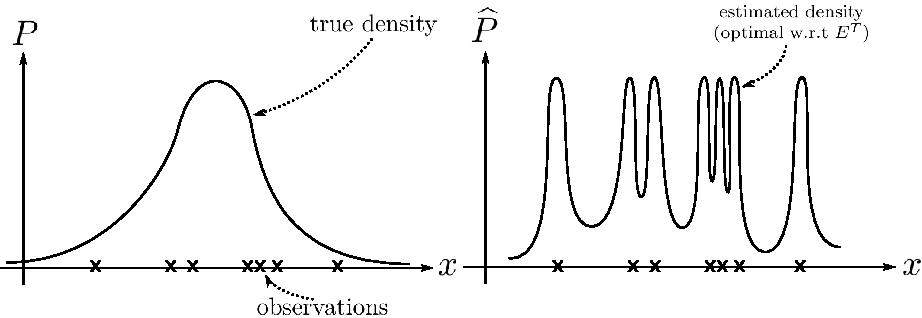
\includegraphics[width=0.8\textwidth]{img/section1_fig3}
\end{center}

\end{frame}
